\subsection{Torus magnet}
\label{torus}
Describe general operational functions, magnetic field. Assembly accuracy.
1 Figure for structure, 1 Figure magnetic field
\vspace{0.3cm}\noindent
\begin{figure}[h]
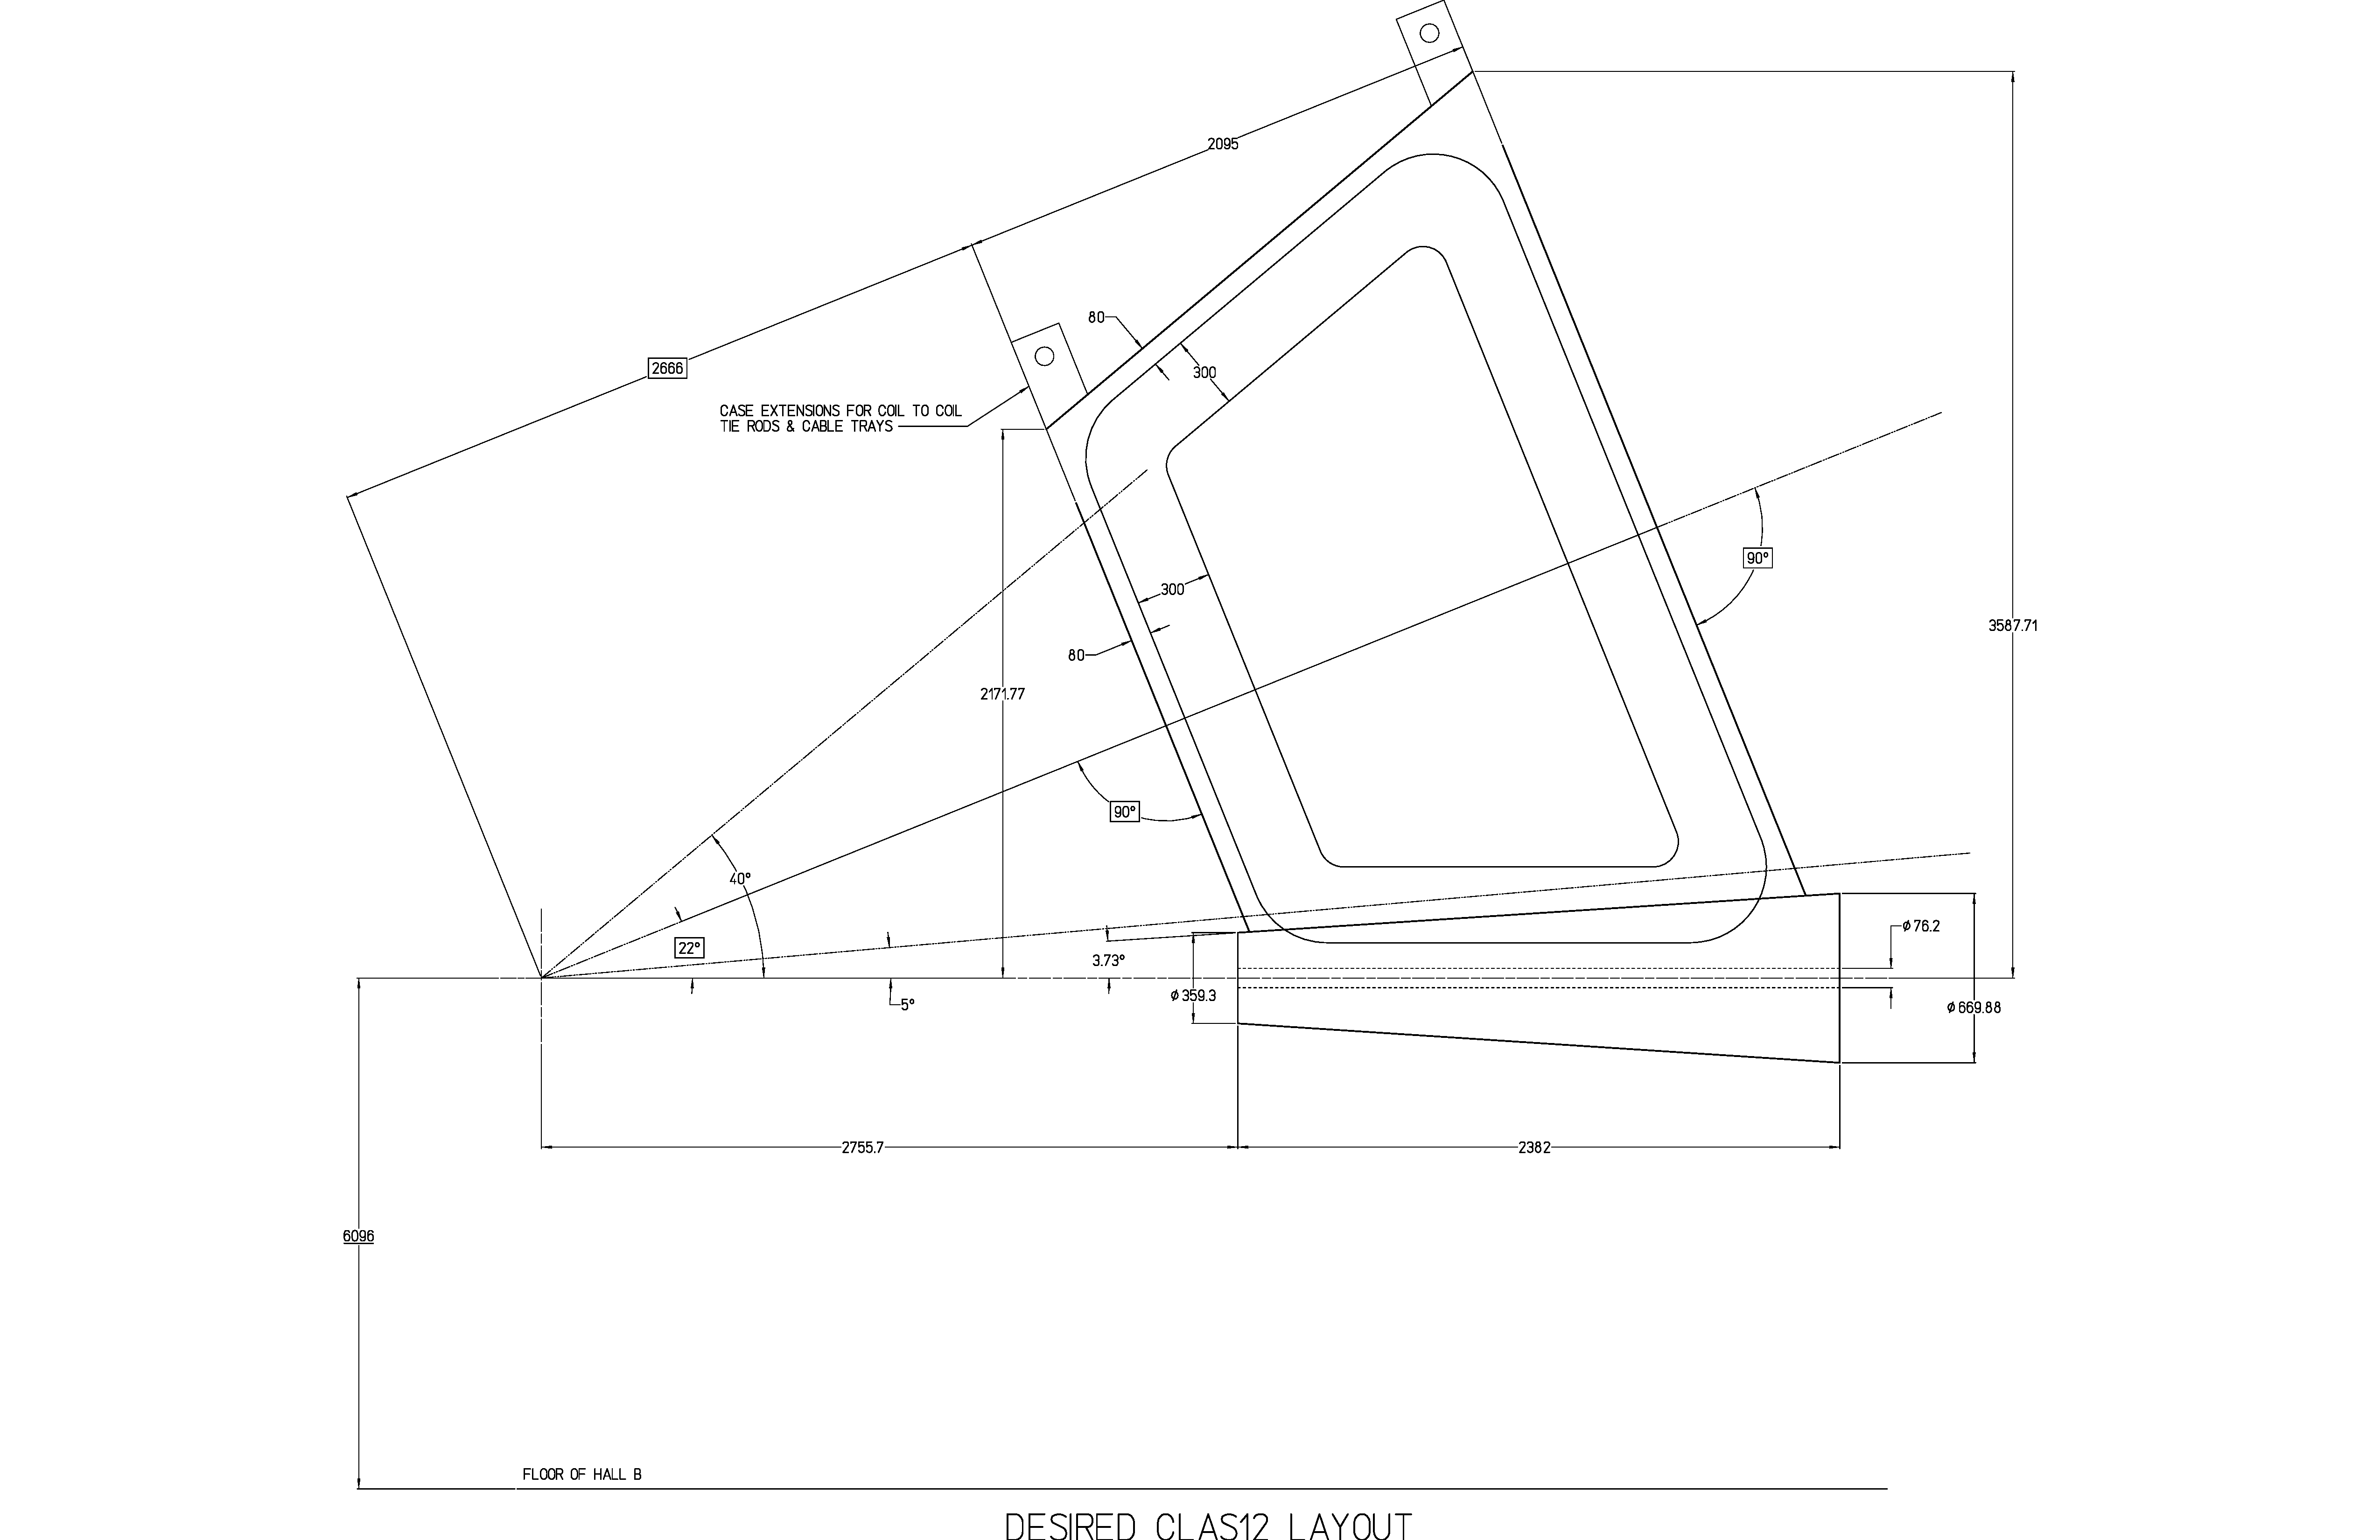
\includegraphics[width=0.6\columnwidth]{clas12_desired.pdf}
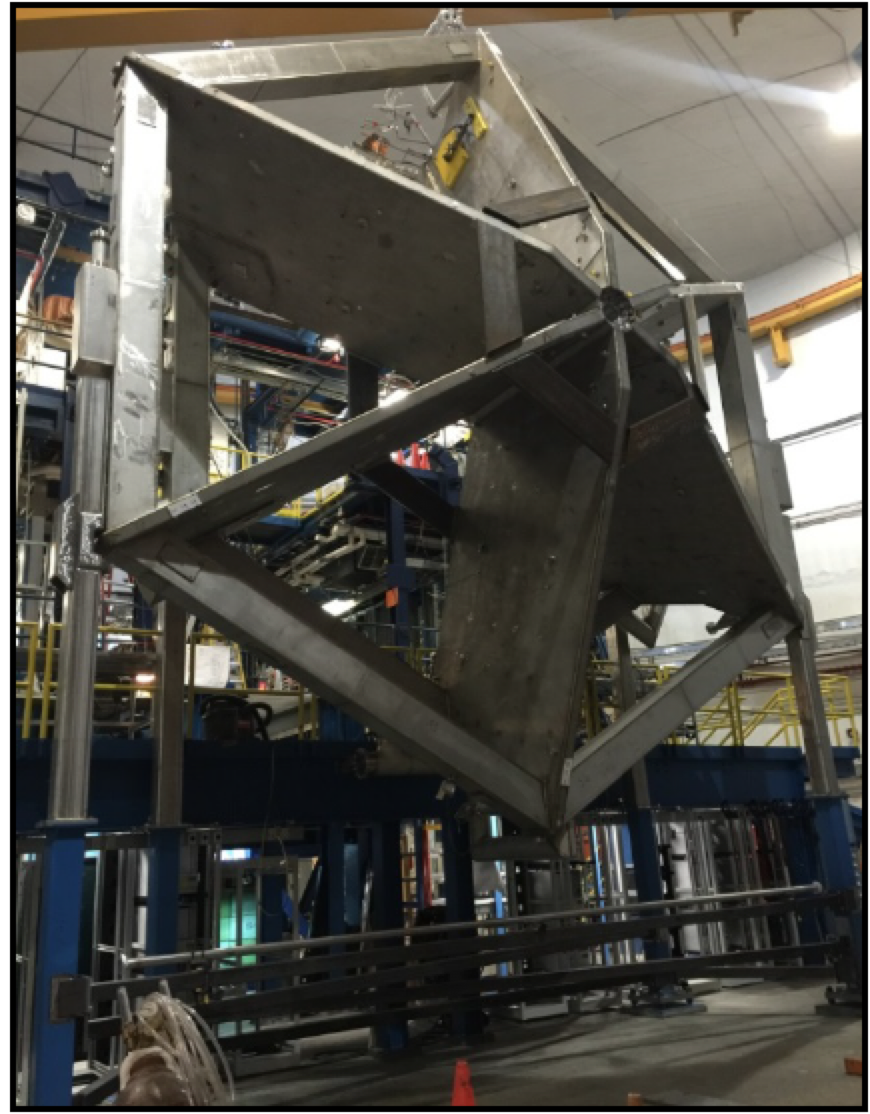
\includegraphics[width=0.35\columnwidth]{Torus-pic.png}
\caption{Left: The shape and dimensions of one of the Torus coils (may not be the final coil shape).
The other five coils are arranged in intervals of $\Delta{\phi} = 60^\circ$ relative the coil mid plane.
Right: The Torus magnet with all six coils assembles in the common cryostat. The coil cryostat width is 120mm. It
has been minimized for maximum acceptance. The braces shown between the coils are removed in the final magnet. }
\end{figure}
%\vfill\eject
\vspace{3cm}



\subsection{Solenoid Magnet}
\label{solenoid}
\vspace{0.3cm}\noindent

\begin{figure}[h]
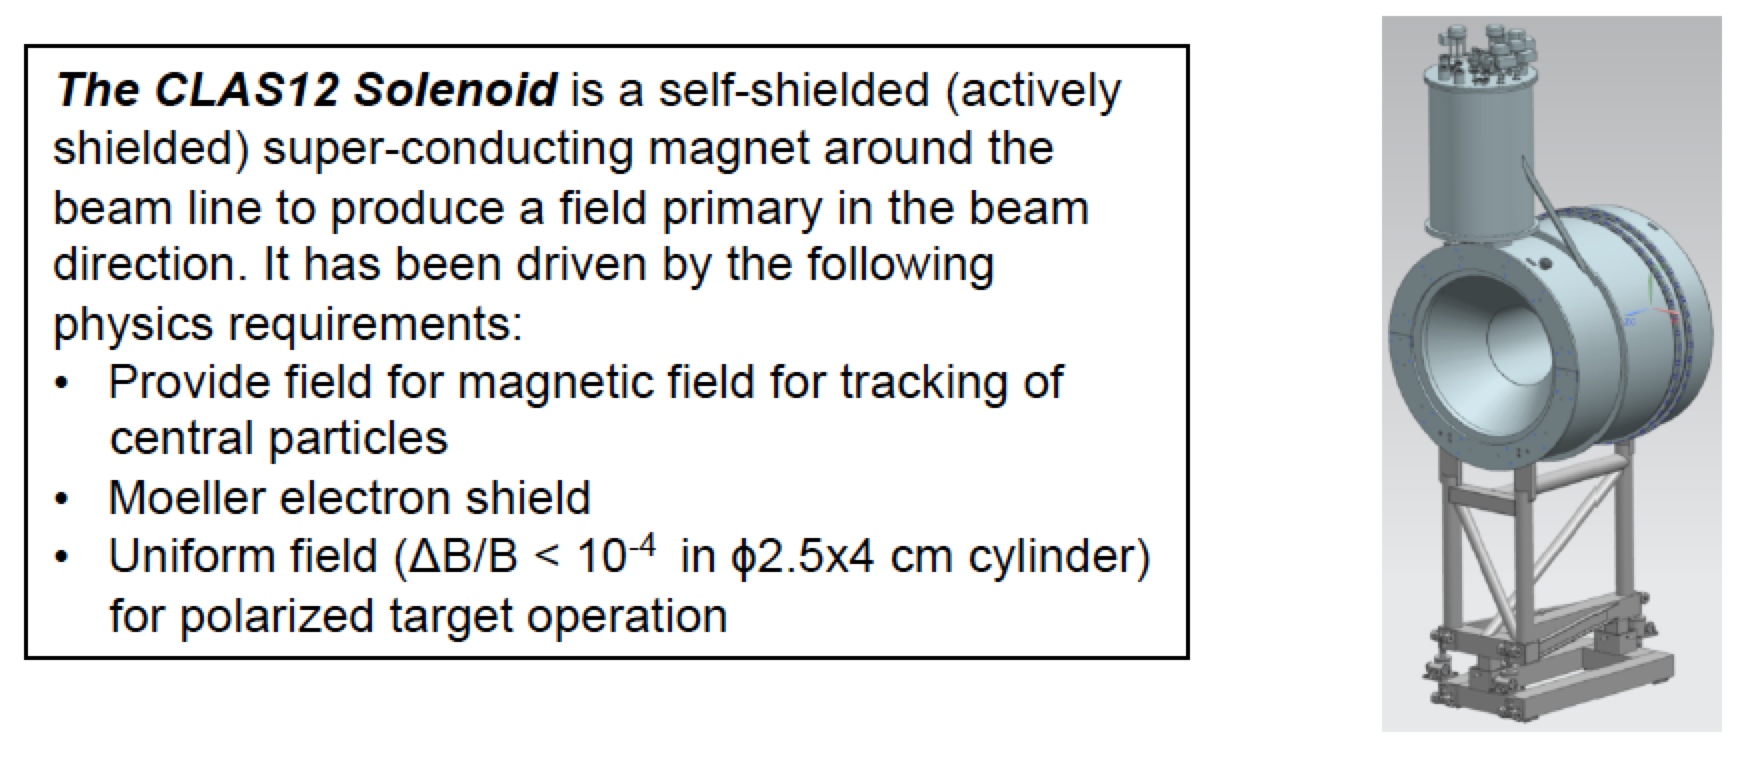
\includegraphics[width=1.0\columnwidth]{Solenoid-pic.png}
\caption{The solenoid magnet is a self-shielded superconducting magnet around the beam beam line
to produce a field primary in the beam direction. It is driven by the physics requirements to 1) provide
a magnetic field for particle tracking, to act as a Moller electron shield, and to provide
a highly uniform field of in the magnet center for operation of a polarized target}
\end{figure}

Described the general design features and 3 operational functions (background shielding,
momentum analysis, polarized target operation.
Solenoid magnet (1 Fig)
Magnetic field description (1 Fig)
%\vspace{0.3cm}\noindent
